\documentclass[twoside]{book}

% Packages required by doxygen
\usepackage{fixltx2e}
\usepackage{calc}
\usepackage{doxygen}
\usepackage[export]{adjustbox} % also loads graphicx
\usepackage{graphicx}
\usepackage[utf8]{inputenc}
\usepackage{makeidx}
\usepackage{multicol}
\usepackage{multirow}
\PassOptionsToPackage{warn}{textcomp}
\usepackage{textcomp}
\usepackage[nointegrals]{wasysym}
\usepackage[table]{xcolor}

% Font selection
\usepackage[T1]{fontenc}
\usepackage[scaled=.90]{helvet}
\usepackage{courier}
\usepackage{amssymb}
\usepackage{sectsty}
\renewcommand{\familydefault}{\sfdefault}
\allsectionsfont{%
  \fontseries{bc}\selectfont%
  \color{darkgray}%
}
\renewcommand{\DoxyLabelFont}{%
  \fontseries{bc}\selectfont%
  \color{darkgray}%
}
\newcommand{\+}{\discretionary{\mbox{\scriptsize$\hookleftarrow$}}{}{}}

% Page & text layout
\usepackage{geometry}
\geometry{%
  a4paper,%
  top=2.5cm,%
  bottom=2.5cm,%
  left=2.5cm,%
  right=2.5cm%
}
\tolerance=750
\hfuzz=15pt
\hbadness=750
\setlength{\emergencystretch}{15pt}
\setlength{\parindent}{0cm}
\setlength{\parskip}{0.2cm}
\makeatletter
\renewcommand{\paragraph}{%
  \@startsection{paragraph}{4}{0ex}{-1.0ex}{1.0ex}{%
    \normalfont\normalsize\bfseries\SS@parafont%
  }%
}
\renewcommand{\subparagraph}{%
  \@startsection{subparagraph}{5}{0ex}{-1.0ex}{1.0ex}{%
    \normalfont\normalsize\bfseries\SS@subparafont%
  }%
}
\makeatother

% Headers & footers
\usepackage{fancyhdr}
\pagestyle{fancyplain}
\fancyhead[LE]{\fancyplain{}{\bfseries\thepage}}
\fancyhead[CE]{\fancyplain{}{}}
\fancyhead[RE]{\fancyplain{}{\bfseries\leftmark}}
\fancyhead[LO]{\fancyplain{}{\bfseries\rightmark}}
\fancyhead[CO]{\fancyplain{}{}}
\fancyhead[RO]{\fancyplain{}{\bfseries\thepage}}
\fancyfoot[LE]{\fancyplain{}{}}
\fancyfoot[CE]{\fancyplain{}{}}
\fancyfoot[RE]{\fancyplain{}{\bfseries\scriptsize Generated on Thu Jan 21 2016 21\+:56\+:28 for Course work by Doxygen }}
\fancyfoot[LO]{\fancyplain{}{\bfseries\scriptsize Generated on Thu Jan 21 2016 21\+:56\+:28 for Course work by Doxygen }}
\fancyfoot[CO]{\fancyplain{}{}}
\fancyfoot[RO]{\fancyplain{}{}}
\renewcommand{\footrulewidth}{0.4pt}
\renewcommand{\chaptermark}[1]{%
  \markboth{#1}{}%
}
\renewcommand{\sectionmark}[1]{%
  \markright{\thesection\ #1}%
}

% Indices & bibliography
\usepackage{natbib}
\usepackage[titles]{tocloft}
\setcounter{tocdepth}{3}
\setcounter{secnumdepth}{5}
\makeindex

% Hyperlinks (required, but should be loaded last)
\usepackage{ifpdf}
\ifpdf
  \usepackage[pdftex,pagebackref=true]{hyperref}
\else
  \usepackage[ps2pdf,pagebackref=true]{hyperref}
\fi
\hypersetup{%
  colorlinks=true,%
  linkcolor=blue,%
  citecolor=blue,%
  unicode%
}

% Custom commands
\newcommand{\clearemptydoublepage}{%
  \newpage{\pagestyle{empty}\cleardoublepage}%
}


%===== C O N T E N T S =====

\begin{document}

% Titlepage & ToC
\hypersetup{pageanchor=false,
             bookmarks=true,
             bookmarksnumbered=true,
             pdfencoding=unicode
            }
\pagenumbering{roman}
\begin{titlepage}
\vspace*{7cm}
\begin{center}%
{\Large Course work }\\
\vspace*{1cm}
{\large Generated by Doxygen 1.8.10}\\
\vspace*{0.5cm}
{\small Thu Jan 21 2016 21:56:28}\\
\end{center}
\end{titlepage}
\clearemptydoublepage
\tableofcontents
\clearemptydoublepage
\pagenumbering{arabic}
\hypersetup{pageanchor=true}

%--- Begin generated contents ---
\chapter{Course Work -\/ I\+M\+A\+T2605}
\label{index}\hypertarget{index}{}\hypertarget{index_intro_sec}{}\section{Introduction}\label{index_intro_sec}
This is the introduction.\hypertarget{index_install_sec}{}\section{Installation}\label{index_install_sec}
\hypertarget{index_step1}{}\subsection{Step 1\+: Opening the box}\label{index_step1}
etc... 
\chapter{Hierarchical Index}
\section{Class Hierarchy}
This inheritance list is sorted roughly, but not completely, alphabetically\+:\begin{DoxyCompactList}
\item \contentsline{section}{rapidxml\+:\+:attribute\+\_\+iterator$<$ Ch $>$}{\pageref{classrapidxml_1_1attribute__iterator}}{}
\item \contentsline{section}{Collidable\+Factory}{\pageref{class_collidable_factory}}{}
\item Drawable\begin{DoxyCompactList}
\item \contentsline{section}{Collidable}{\pageref{class_collidable}}{}
\begin{DoxyCompactList}
\item \contentsline{section}{Circle}{\pageref{class_circle}}{}
\begin{DoxyCompactList}
\item \contentsline{section}{Tyre}{\pageref{class_tyre}}{}
\end{DoxyCompactList}
\item \contentsline{section}{O\+B\+B}{\pageref{class_o_b_b}}{}
\begin{DoxyCompactList}
\item \contentsline{section}{Box}{\pageref{class_box}}{}
\item \contentsline{section}{Car}{\pageref{class_car}}{}
\end{DoxyCompactList}
\end{DoxyCompactList}
\item \contentsline{section}{Game}{\pageref{class_game}}{}
\end{DoxyCompactList}
\item exception\begin{DoxyCompactList}
\item \contentsline{section}{rapidxml\+:\+:parse\+\_\+error}{\pageref{classrapidxml_1_1parse__error}}{}
\end{DoxyCompactList}
\item \contentsline{section}{rapidxml\+:\+:file$<$ Ch $>$}{\pageref{classrapidxml_1_1file}}{}
\item \contentsline{section}{rapidxml\+:\+:memory\+\_\+pool$<$ Ch $>$}{\pageref{classrapidxml_1_1memory__pool}}{}
\begin{DoxyCompactList}
\item \contentsline{section}{rapidxml\+:\+:xml\+\_\+document$<$ Ch $>$}{\pageref{classrapidxml_1_1xml__document}}{}
\end{DoxyCompactList}
\item \contentsline{section}{rapidxml\+:\+:node\+\_\+iterator$<$ Ch $>$}{\pageref{classrapidxml_1_1node__iterator}}{}
\item \contentsline{section}{Vector2\+D$<$ G $>$}{\pageref{class_vector2_d}}{}
\item \contentsline{section}{Vector2\+D$<$ double $>$}{\pageref{class_vector2_d}}{}
\item \contentsline{section}{rapidxml\+:\+:xml\+\_\+base$<$ Ch $>$}{\pageref{classrapidxml_1_1xml__base}}{}
\begin{DoxyCompactList}
\item \contentsline{section}{rapidxml\+:\+:xml\+\_\+attribute$<$ Ch $>$}{\pageref{classrapidxml_1_1xml__attribute}}{}
\item \contentsline{section}{rapidxml\+:\+:xml\+\_\+node$<$ Ch $>$}{\pageref{classrapidxml_1_1xml__node}}{}
\begin{DoxyCompactList}
\item \contentsline{section}{rapidxml\+:\+:xml\+\_\+document$<$ Ch $>$}{\pageref{classrapidxml_1_1xml__document}}{}
\end{DoxyCompactList}
\end{DoxyCompactList}
\end{DoxyCompactList}

\chapter{Class Index}
\section{Class List}
Here are the classes, structs, unions and interfaces with brief descriptions\+:\begin{DoxyCompactList}
\item\contentsline{section}{\hyperlink{classrapidxml_1_1attribute__iterator}{rapidxml\+::attribute\+\_\+iterator$<$ Ch $>$} \\*Iterator of child attributes of \hyperlink{classrapidxml_1_1xml__node}{xml\+\_\+node} }{\pageref{classrapidxml_1_1attribute__iterator}}{}
\item\contentsline{section}{\hyperlink{class_box}{Box} \\*\hyperlink{class_box}{Box} to be used as collidable obstacle in the game }{\pageref{class_box}}{}
\item\contentsline{section}{\hyperlink{class_car}{Car} }{\pageref{class_car}}{}
\item\contentsline{section}{\hyperlink{class_circle}{Circle} \\*Circular collidables to be used in the game }{\pageref{class_circle}}{}
\item\contentsline{section}{\hyperlink{class_collidable}{Collidable} \\*Base class for every collidable object in the game }{\pageref{class_collidable}}{}
\item\contentsline{section}{\hyperlink{class_collidable_factory}{Collidable\+Factory} }{\pageref{class_collidable_factory}}{}
\item\contentsline{section}{\hyperlink{classrapidxml_1_1file}{rapidxml\+::file$<$ Ch $>$} \\*Represents data loaded from a file }{\pageref{classrapidxml_1_1file}}{}
\item\contentsline{section}{\hyperlink{class_game}{Game} }{\pageref{class_game}}{}
\item\contentsline{section}{\hyperlink{classrapidxml_1_1memory__pool}{rapidxml\+::memory\+\_\+pool$<$ Ch $>$} }{\pageref{classrapidxml_1_1memory__pool}}{}
\item\contentsline{section}{\hyperlink{classrapidxml_1_1node__iterator}{rapidxml\+::node\+\_\+iterator$<$ Ch $>$} \\*Iterator of child nodes of \hyperlink{classrapidxml_1_1xml__node}{xml\+\_\+node} }{\pageref{classrapidxml_1_1node__iterator}}{}
\item\contentsline{section}{\hyperlink{class_o_b_b}{O\+B\+B} }{\pageref{class_o_b_b}}{}
\item\contentsline{section}{\hyperlink{classrapidxml_1_1parse__error}{rapidxml\+::parse\+\_\+error} }{\pageref{classrapidxml_1_1parse__error}}{}
\item\contentsline{section}{\hyperlink{class_tyre}{Tyre} \\*\hyperlink{class_tyre}{Tyre} to be used as collidable obstacle in the game }{\pageref{class_tyre}}{}
\item\contentsline{section}{\hyperlink{class_vector2_d}{Vector2\+D$<$ G $>$} \\*Small text that appears on Classes page }{\pageref{class_vector2_d}}{}
\item\contentsline{section}{\hyperlink{classrapidxml_1_1xml__attribute}{rapidxml\+::xml\+\_\+attribute$<$ Ch $>$} }{\pageref{classrapidxml_1_1xml__attribute}}{}
\item\contentsline{section}{\hyperlink{classrapidxml_1_1xml__base}{rapidxml\+::xml\+\_\+base$<$ Ch $>$} }{\pageref{classrapidxml_1_1xml__base}}{}
\item\contentsline{section}{\hyperlink{classrapidxml_1_1xml__document}{rapidxml\+::xml\+\_\+document$<$ Ch $>$} }{\pageref{classrapidxml_1_1xml__document}}{}
\item\contentsline{section}{\hyperlink{classrapidxml_1_1xml__node}{rapidxml\+::xml\+\_\+node$<$ Ch $>$} }{\pageref{classrapidxml_1_1xml__node}}{}
\end{DoxyCompactList}

\chapter{File Index}
\section{File List}
Here is a list of all documented files with brief descriptions\+:\begin{DoxyCompactList}
\item\contentsline{section}{C\+:/\+Users/\+Vitor/\+Documents/\+Visual Studio 2013/\+Projects/\+Course\+Work/coursework/include/{\bfseries car.\+h} }{\pageref{car_8h}}{}
\item\contentsline{section}{C\+:/\+Users/\+Vitor/\+Documents/\+Visual Studio 2013/\+Projects/\+Course\+Work/coursework/include/{\bfseries circle.\+h} }{\pageref{circle_8h}}{}
\item\contentsline{section}{C\+:/\+Users/\+Vitor/\+Documents/\+Visual Studio 2013/\+Projects/\+Course\+Work/coursework/include/\hyperlink{collidable_8h}{collidable.\+h} }{\pageref{collidable_8h}}{}
\item\contentsline{section}{C\+:/\+Users/\+Vitor/\+Documents/\+Visual Studio 2013/\+Projects/\+Course\+Work/coursework/include/{\bfseries collision.\+h} }{\pageref{collision_8h}}{}
\item\contentsline{section}{C\+:/\+Users/\+Vitor/\+Documents/\+Visual Studio 2013/\+Projects/\+Course\+Work/coursework/include/\hyperlink{game_8h}{game.\+h} }{\pageref{game_8h}}{}
\item\contentsline{section}{C\+:/\+Users/\+Vitor/\+Documents/\+Visual Studio 2013/\+Projects/\+Course\+Work/coursework/include/{\bfseries obb.\+h} }{\pageref{obb_8h}}{}
\item\contentsline{section}{C\+:/\+Users/\+Vitor/\+Documents/\+Visual Studio 2013/\+Projects/\+Course\+Work/coursework/include/\hyperlink{vector2_d_8h}{vector2\+D.\+h} }{\pageref{vector2_d_8h}}{}
\item\contentsline{section}{C\+:/\+Users/\+Vitor/\+Documents/\+Visual Studio 2013/\+Projects/\+Course\+Work/coursework/src/\hyperlink{game_8cpp}{game.\+cpp} }{\pageref{game_8cpp}}{}
\item\contentsline{section}{C\+:/\+Users/\+Vitor/\+Documents/\+Visual Studio 2013/\+Projects/\+Course\+Work/coursework/src/\hyperlink{main_8cpp}{main.\+cpp} }{\pageref{main_8cpp}}{}
\end{DoxyCompactList}

\chapter{Class Documentation}
\hypertarget{class_car}{}\section{Car Class Reference}
\label{class_car}\index{Car@{Car}}
Inheritance diagram for Car\+:\begin{figure}[H]
\begin{center}
\leavevmode
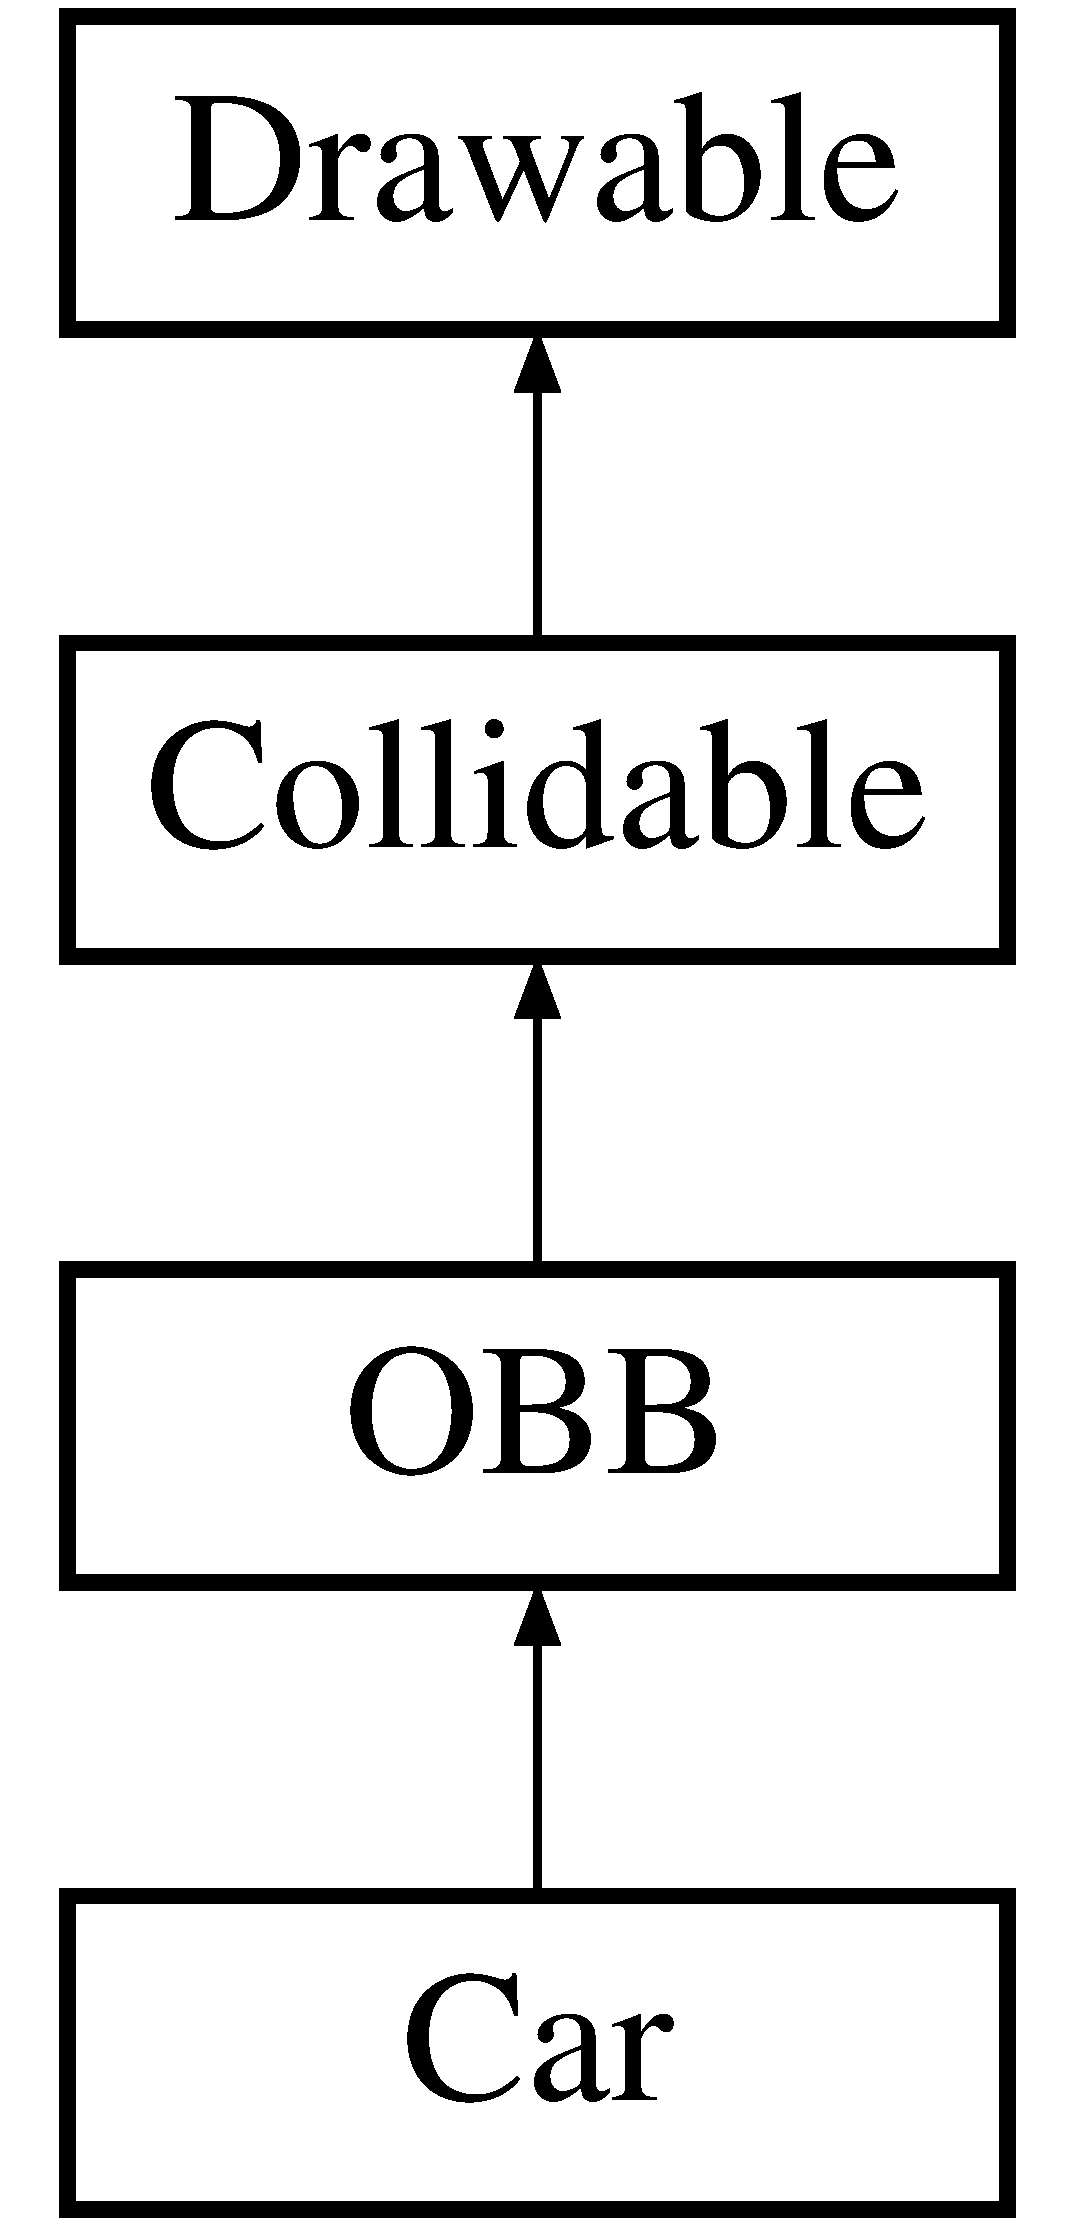
\includegraphics[height=4.000000cm]{class_car}
\end{center}
\end{figure}
\subsection*{Public Member Functions}
\begin{DoxyCompactItemize}
\item 
\hypertarget{class_car_abf11f99802806a2fe70fefb90173a98f}{}{\bfseries Car} (double d\+Pos\+X, double d\+Pos\+Y, double d\+Half\+Extent\+X, double d\+Half\+Extent\+Y, double d\+Angle)\label{class_car_abf11f99802806a2fe70fefb90173a98f}

\item 
\hypertarget{class_car_ab7860fcfd5e75787d358128e04442464}{}void {\bfseries update} (float elapsed)\label{class_car_ab7860fcfd5e75787d358128e04442464}

\item 
\hypertarget{class_car_ad8fce46167e6bdbb9f91ca8669da63e3}{}void {\bfseries set\+Angle} (double angle)\label{class_car_ad8fce46167e6bdbb9f91ca8669da63e3}

\end{DoxyCompactItemize}
\subsection*{Additional Inherited Members}


The documentation for this class was generated from the following files\+:\begin{DoxyCompactItemize}
\item 
include/car.\+h\item 
src/car.\+cpp\end{DoxyCompactItemize}

\hypertarget{class_circle}{}\section{Circle Class Reference}
\label{class_circle}\index{Circle@{Circle}}
Inheritance diagram for Circle\+:\begin{figure}[H]
\begin{center}
\leavevmode
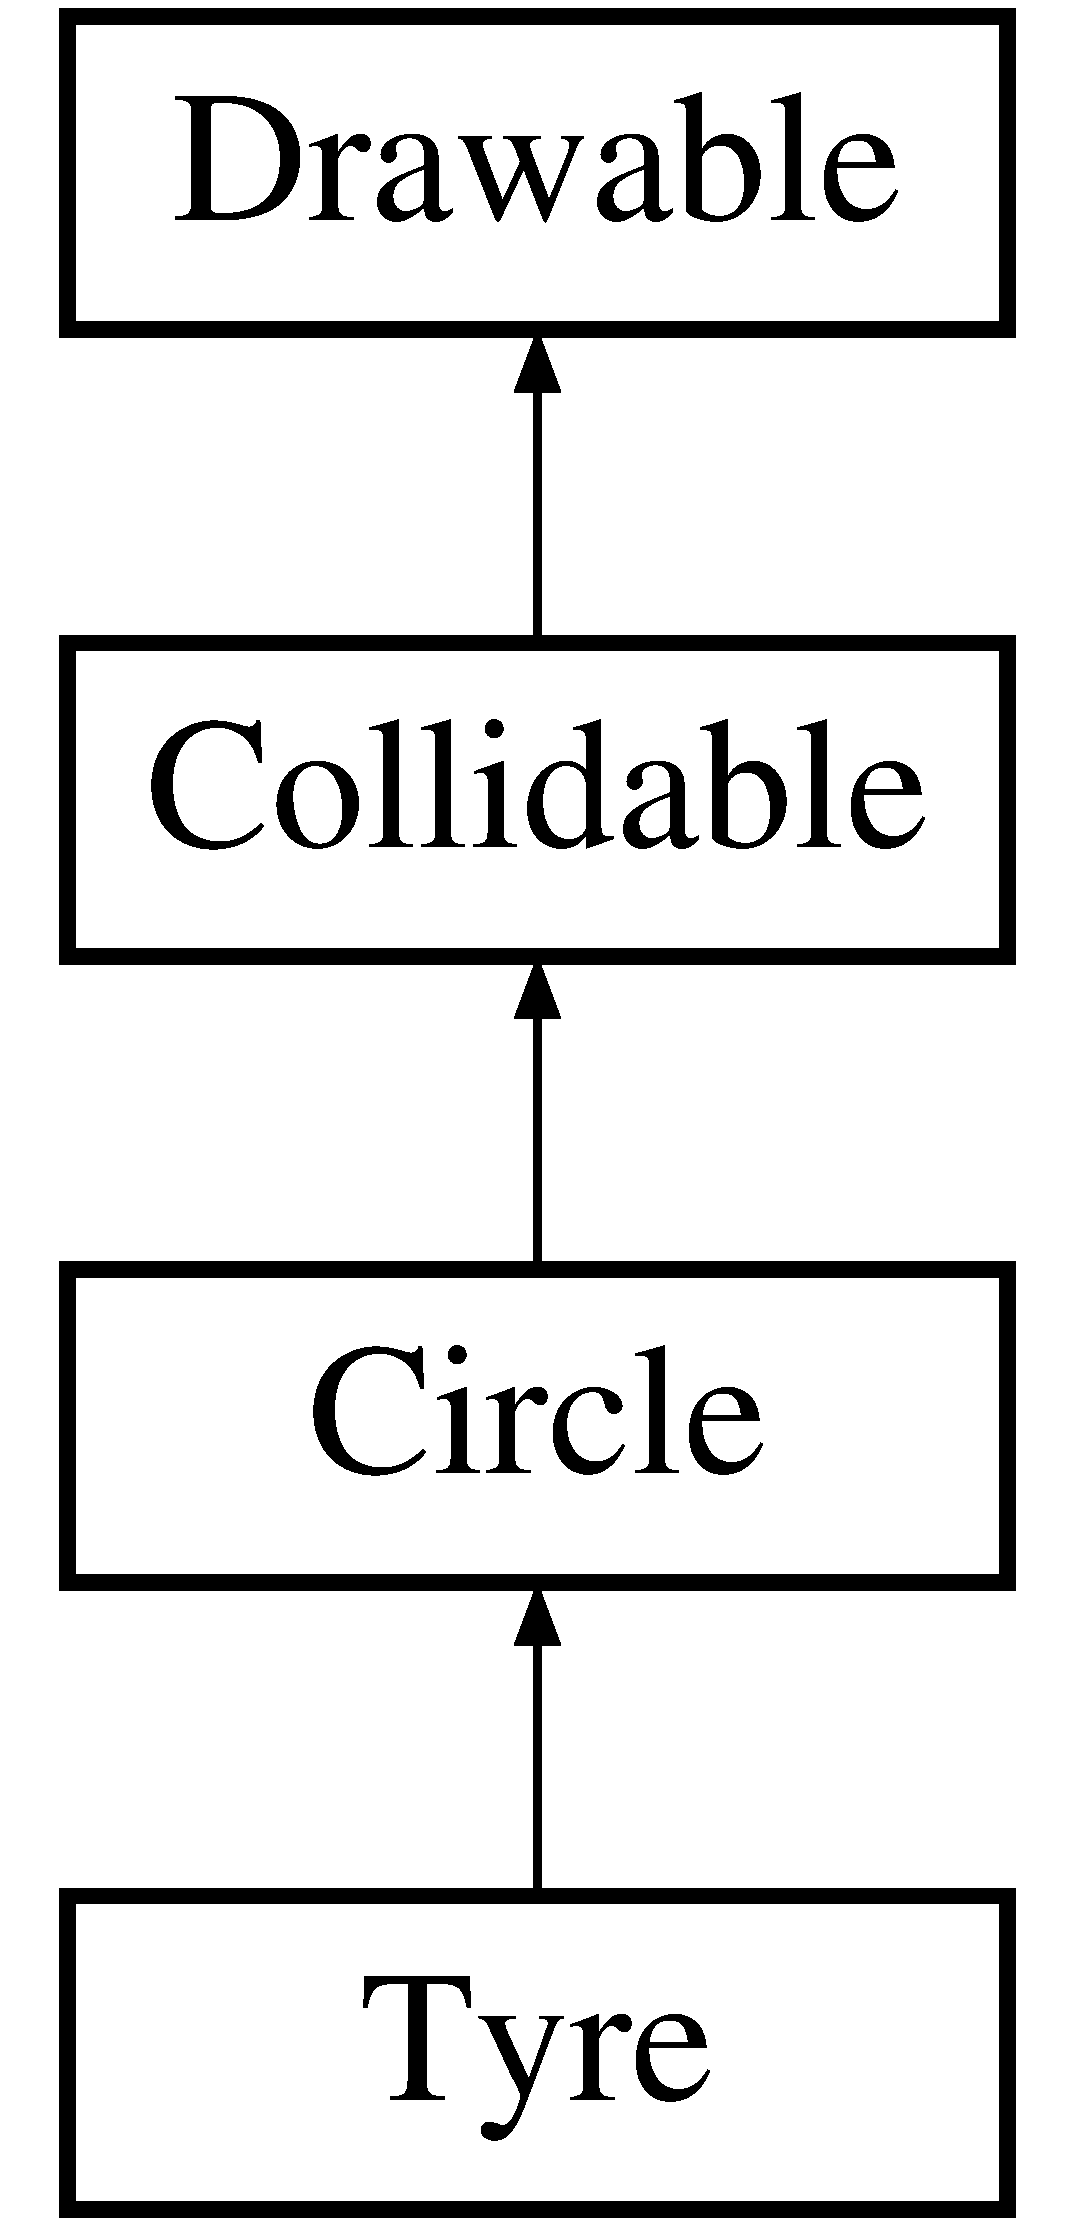
\includegraphics[height=4.000000cm]{class_circle}
\end{center}
\end{figure}
\subsection*{Public Member Functions}
\begin{DoxyCompactItemize}
\item 
\hypertarget{class_circle_ac69dcf84ea92b1ea85880b15d83bcea5}{}{\bfseries Circle} (double f\+Pos\+X, double f\+Pos\+Y, double f\+Radius, double f\+Orientation)\label{class_circle_ac69dcf84ea92b1ea85880b15d83bcea5}

\item 
\hypertarget{class_circle_afe23c30a1bbc5e831b72063aef91b38f}{}void {\bfseries update\+Points} ()\label{class_circle_afe23c30a1bbc5e831b72063aef91b38f}

\item 
\hypertarget{class_circle_a7b23c1ed107b8a309fc1c5d0f6635ae9}{}void \hyperlink{class_circle_a7b23c1ed107b8a309fc1c5d0f6635ae9}{check\+Collision} (\hyperlink{class_collidable}{Collidable} $\ast$collidable)\label{class_circle_a7b23c1ed107b8a309fc1c5d0f6635ae9}

\begin{DoxyCompactList}\small\item\em Virtual method to check collision with another \hyperlink{class_collidable}{Collidable} object. \end{DoxyCompactList}\item 
\hypertarget{class_circle_ad528dfc586b5a46b11401abf52d8da87}{}void \hyperlink{class_circle_ad528dfc586b5a46b11401abf52d8da87}{check\+Collision} (\hyperlink{class_circle}{Circle} $\ast$circle)\label{class_circle_ad528dfc586b5a46b11401abf52d8da87}

\begin{DoxyCompactList}\small\item\em Virtual method to check collision with a \hyperlink{class_circle}{Circle} object. \end{DoxyCompactList}\item 
\hypertarget{class_circle_a328f1400d819209db7b64431b60bbc59}{}void \hyperlink{class_circle_a328f1400d819209db7b64431b60bbc59}{check\+Collision} (\hyperlink{class_o_b_b}{O\+B\+B} $\ast$obb)\label{class_circle_a328f1400d819209db7b64431b60bbc59}

\begin{DoxyCompactList}\small\item\em Virtual method to check collision with an \hyperlink{class_o_b_b}{O\+B\+B} object. \end{DoxyCompactList}\item 
\hypertarget{class_circle_ac6c48964ac829b4c1a15b313d9ae102a}{}void {\bfseries set\+Texture} (sf\+::\+Texture $\ast$texture)\label{class_circle_ac6c48964ac829b4c1a15b313d9ae102a}

\end{DoxyCompactItemize}
\subsection*{Additional Inherited Members}


The documentation for this class was generated from the following files\+:\begin{DoxyCompactItemize}
\item 
C\+:/\+Users/\+Vitor/\+Documents/\+Visual Studio 2013/\+Projects/\+Course\+Work/coursework/include/circle.\+h\item 
C\+:/\+Users/\+Vitor/\+Documents/\+Visual Studio 2013/\+Projects/\+Course\+Work/coursework/src/circle.\+cpp\end{DoxyCompactItemize}

\hypertarget{class_collidable}{}\section{Collidable Class Reference}
\label{class_collidable}\index{Collidable@{Collidable}}
Inheritance diagram for Collidable\+:\begin{figure}[H]
\begin{center}
\leavevmode
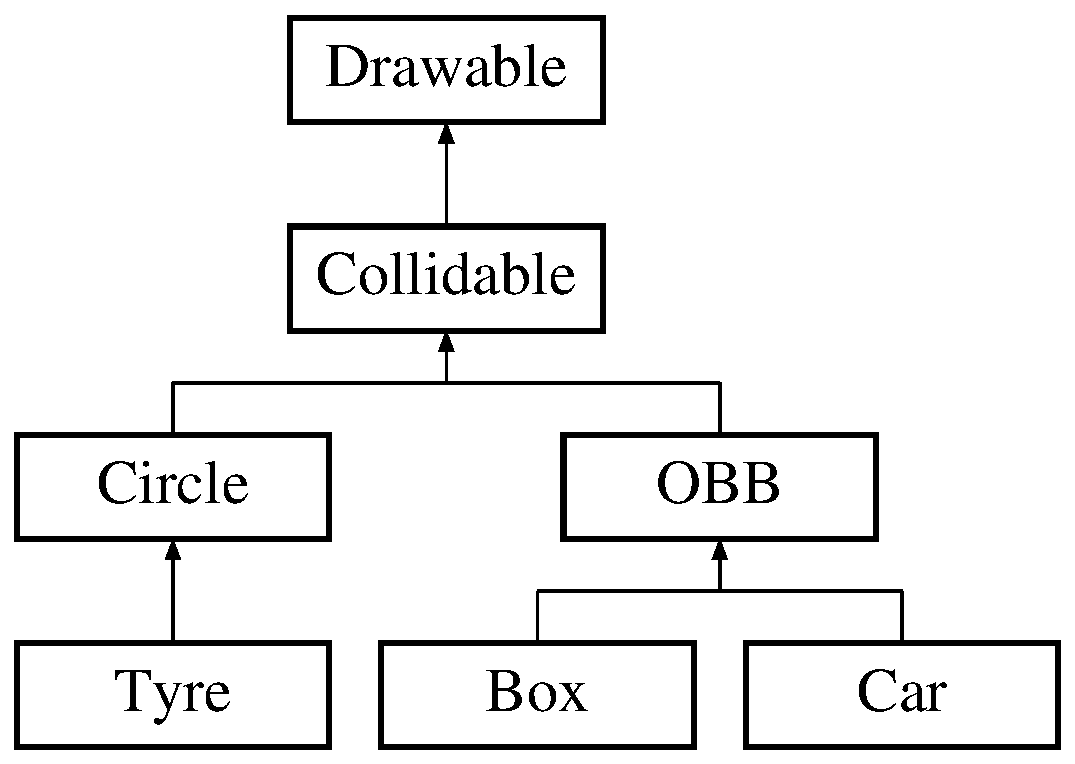
\includegraphics[height=4.000000cm]{class_collidable}
\end{center}
\end{figure}
\subsection*{Public Member Functions}
\begin{DoxyCompactItemize}
\item 
\hypertarget{class_collidable_ad5022811d28d0db8a58e4ecfda914f4b}{}\hyperlink{class_vector2_d}{Vector2\+D}$<$ double $>$ {\bfseries get\+Position} ()\label{class_collidable_ad5022811d28d0db8a58e4ecfda914f4b}

\item 
\hypertarget{class_collidable_abfdcd815a5f8aabd860e2b69bc4bea21}{}\hyperlink{class_vector2_d}{Vector2\+D}$<$ double $>$ {\bfseries get\+Velocity} ()\label{class_collidable_abfdcd815a5f8aabd860e2b69bc4bea21}

\item 
\hypertarget{class_collidable_ac6387b72fd5e194cd3e38cf22e30e75a}{}\hyperlink{class_vector2_d}{Vector2\+D}$<$ double $>$ {\bfseries get\+Acceleration} ()\label{class_collidable_ac6387b72fd5e194cd3e38cf22e30e75a}

\item 
\hypertarget{class_collidable_a3ceb05fc466651c75f1c23231a9cf7a9}{}double {\bfseries get\+Inverse\+Mass} ()\label{class_collidable_a3ceb05fc466651c75f1c23231a9cf7a9}

\item 
\hypertarget{class_collidable_aee9547a28db55d503164cdf5f3d069fc}{}double {\bfseries get\+Angle} ()\label{class_collidable_aee9547a28db55d503164cdf5f3d069fc}

\item 
\hypertarget{class_collidable_af00403ad8cd4daf89cc38653f7cb8176}{}void {\bfseries accelerate} ()\label{class_collidable_af00403ad8cd4daf89cc38653f7cb8176}

\item 
\hypertarget{class_collidable_a387fbafb5027cd3d53578aadd2838e38}{}void {\bfseries decelerate} ()\label{class_collidable_a387fbafb5027cd3d53578aadd2838e38}

\item 
\hypertarget{class_collidable_abd76296323992091a7e1f5a15c82861c}{}void {\bfseries reverse} ()\label{class_collidable_abd76296323992091a7e1f5a15c82861c}

\item 
\hypertarget{class_collidable_aad6377534a6dd68073a0d4283c9349fc}{}void {\bfseries turn\+Right} ()\label{class_collidable_aad6377534a6dd68073a0d4283c9349fc}

\item 
\hypertarget{class_collidable_a807824d4a255e9d0c48464a6f67e9837}{}void {\bfseries turn\+Left} ()\label{class_collidable_a807824d4a255e9d0c48464a6f67e9837}

\item 
\hypertarget{class_collidable_ab4a89fa87f6e2ea151c5e8c9e80847b3}{}void {\bfseries set\+Position} (\hyperlink{class_vector2_d}{Vector2\+D}$<$ double $>$ position)\label{class_collidable_ab4a89fa87f6e2ea151c5e8c9e80847b3}

\item 
\hypertarget{class_collidable_a3b218cc8ee1f40a5cfce42b764615ac6}{}void {\bfseries set\+Velocity} (\hyperlink{class_vector2_d}{Vector2\+D}$<$ double $>$ velocity)\label{class_collidable_a3b218cc8ee1f40a5cfce42b764615ac6}

\end{DoxyCompactItemize}
\subsection*{Protected Attributes}
\begin{DoxyCompactItemize}
\item 
\hypertarget{class_collidable_aa9b3dd6f54428c0e538eb75a5166dd93}{}\hyperlink{class_vector2_d}{Vector2\+D}$<$ double $>$ {\bfseries m\+\_\+dv\+Position}\label{class_collidable_aa9b3dd6f54428c0e538eb75a5166dd93}

\item 
\hypertarget{class_collidable_ab7f405cb0f44372741baff129eabb8a8}{}\hyperlink{class_vector2_d}{Vector2\+D}$<$ double $>$ {\bfseries m\+\_\+dv\+Velocity}\label{class_collidable_ab7f405cb0f44372741baff129eabb8a8}

\item 
\hypertarget{class_collidable_abda695eecdb275f43bdb9fce1f58ef09}{}\hyperlink{class_vector2_d}{Vector2\+D}$<$ double $>$ {\bfseries m\+\_\+dv\+Acceleration}\label{class_collidable_abda695eecdb275f43bdb9fce1f58ef09}

\item 
\hypertarget{class_collidable_aa8bc9d03ab2be264b819053f347c432a}{}\hyperlink{class_vector2_d}{Vector2\+D}$<$ double $>$ {\bfseries m\+\_\+dv\+Thrust}\label{class_collidable_aa8bc9d03ab2be264b819053f347c432a}

\item 
\hypertarget{class_collidable_a69d06f98760bca141c613a4f4f256a5d}{}double {\bfseries m\+\_\+d\+Force}\label{class_collidable_a69d06f98760bca141c613a4f4f256a5d}

\item 
\hypertarget{class_collidable_acf991846cbb2b81c4cee2900c92c9260}{}double {\bfseries m\+\_\+d\+Thrust}\label{class_collidable_acf991846cbb2b81c4cee2900c92c9260}

\item 
\hypertarget{class_collidable_a1e3f4151e4cd0771b24ed0029ff796cb}{}double {\bfseries m\+\_\+d\+Acceleration}\label{class_collidable_a1e3f4151e4cd0771b24ed0029ff796cb}

\item 
\hypertarget{class_collidable_a9253389e228d50dec0a4c0c12bf6e604}{}double {\bfseries m\+\_\+d\+Velocity}\label{class_collidable_a9253389e228d50dec0a4c0c12bf6e604}

\item 
\hypertarget{class_collidable_aa6b2bd9cb61b6f410e94c43e1ae25abc}{}double {\bfseries m\+\_\+d\+Inverse\+Mass}\label{class_collidable_aa6b2bd9cb61b6f410e94c43e1ae25abc}

\item 
\hypertarget{class_collidable_ad3a6769c49a8d2ee0b0434849952dcb2}{}double {\bfseries m\+\_\+d\+Angle}\label{class_collidable_ad3a6769c49a8d2ee0b0434849952dcb2}

\item 
\hypertarget{class_collidable_a13a62d6d9fb69397c5ad03e6ec1c3b2d}{}sf\+::\+Vertex\+Array {\bfseries m\+\_\+va\+Points}\label{class_collidable_a13a62d6d9fb69397c5ad03e6ec1c3b2d}

\end{DoxyCompactItemize}


The documentation for this class was generated from the following files\+:\begin{DoxyCompactItemize}
\item 
include/collidable.\+h\item 
src/collidable.\+cpp\end{DoxyCompactItemize}

\hypertarget{class_collision}{}\section{Collision Class Reference}
\label{class_collision}\index{Collision@{Collision}}
\subsection*{Public Member Functions}
\begin{DoxyCompactItemize}
\item 
\hypertarget{class_collision_afe7999685b8f1886d4dbb2ce43a6bb29}{}void {\bfseries check\+Collision} (\hyperlink{class_o_b_b}{O\+B\+B} $\ast$obb, \hyperlink{class_circle}{Circle} $\ast$circle)\label{class_collision_afe7999685b8f1886d4dbb2ce43a6bb29}

\item 
\hypertarget{class_collision_a486f62260900e934b3776861d6373995}{}void {\bfseries check\+Collision} (\hyperlink{class_circle}{Circle} $\ast$circle, \hyperlink{class_o_b_b}{O\+B\+B} $\ast$obb)\label{class_collision_a486f62260900e934b3776861d6373995}

\item 
\hypertarget{class_collision_a8fcea4d350d740f1578c55cff95ba08f}{}bool {\bfseries check\+Collision} (\hyperlink{class_o_b_b}{O\+B\+B} $\ast$obb1, \hyperlink{class_o_b_b}{O\+B\+B} $\ast$obb2)\label{class_collision_a8fcea4d350d740f1578c55cff95ba08f}

\item 
\hypertarget{class_collision_a14f2ada41144c2df70bd900f95744b6e}{}void {\bfseries check\+Collision} (\hyperlink{class_circle}{Circle} $\ast$circle1, \hyperlink{class_circle}{Circle} $\ast$circle2)\label{class_collision_a14f2ada41144c2df70bd900f95744b6e}

\item 
\hypertarget{class_collision_a4038ffe9c7bfe8cf345871daa905d200}{}void {\bfseries check\+Collision} (\hyperlink{class_collidable}{Collidable} $\ast$collidable1, \hyperlink{class_collidable}{Collidable} $\ast$collidable2)\label{class_collision_a4038ffe9c7bfe8cf345871daa905d200}

\item 
\hypertarget{class_collision_a4b1135376307e6a3d0de0d2b7bb64e68}{}void {\bfseries resolve\+Impulses} (\hyperlink{class_collidable}{Collidable} $\ast$collidable1, \hyperlink{class_collidable}{Collidable} $\ast$collidable2, \hyperlink{class_vector2_d}{Vector2\+D}$<$ double $>$ $\ast$collision\+Normal)\label{class_collision_a4b1135376307e6a3d0de0d2b7bb64e68}

\end{DoxyCompactItemize}


The documentation for this class was generated from the following files\+:\begin{DoxyCompactItemize}
\item 
C\+:/\+Users/\+Vitor/\+Documents/\+Visual Studio 2013/\+Projects/\+Course\+Work/coursework/include/collision.\+h\item 
C\+:/\+Users/\+Vitor/\+Documents/\+Visual Studio 2013/\+Projects/\+Course\+Work/coursework/src/collision.\+cpp\end{DoxyCompactItemize}

\hypertarget{class_game}{}\section{Game Class Reference}
\label{class_game}\index{Game@{Game}}
Inheritance diagram for Game\+:\begin{figure}[H]
\begin{center}
\leavevmode
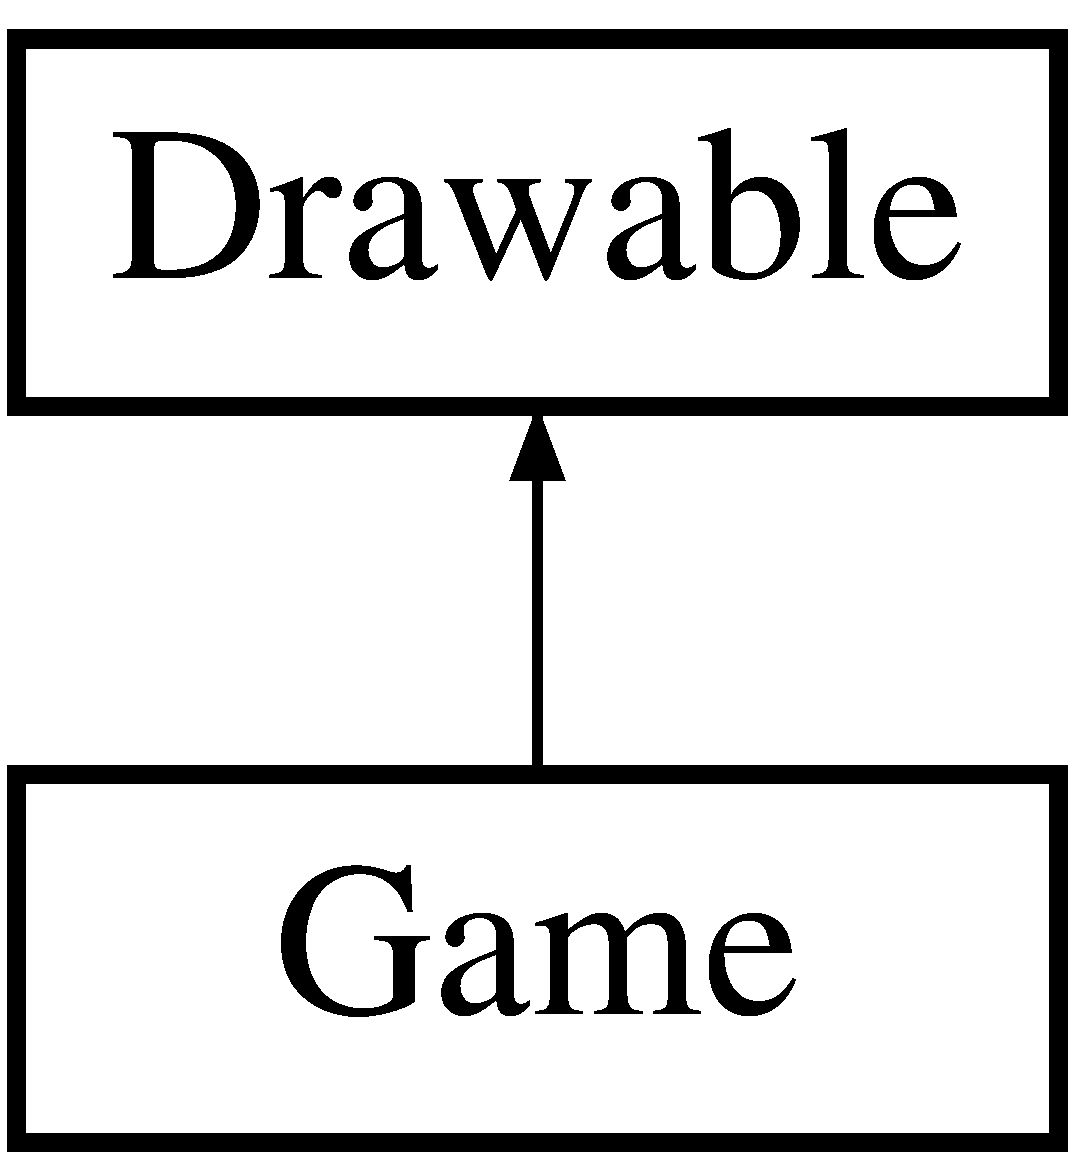
\includegraphics[height=2.000000cm]{class_game}
\end{center}
\end{figure}
\subsection*{Public Member Functions}
\begin{DoxyCompactItemize}
\item 
\hypertarget{class_game_ad59df6562a58a614fda24622d3715b65}{}\hyperlink{class_game_ad59df6562a58a614fda24622d3715b65}{Game} ()\label{class_game_ad59df6562a58a614fda24622d3715b65}

\begin{DoxyCompactList}\small\item\em Constructor. \end{DoxyCompactList}\item 
\hypertarget{class_game_a260c4d5123eb3a51cbd0bb685546cef4}{}void \hyperlink{class_game_a260c4d5123eb3a51cbd0bb685546cef4}{draw} (Render\+Target \&target, Render\+States states) const \label{class_game_a260c4d5123eb3a51cbd0bb685546cef4}

\begin{DoxyCompactList}\small\item\em Draw function (from sf\+::\+Drawable) \end{DoxyCompactList}\item 
\hypertarget{class_game_acc8519c7ced1cf9eb9bbb3a2f325f6a0}{}void \hyperlink{class_game_acc8519c7ced1cf9eb9bbb3a2f325f6a0}{update} (float timestep)\label{class_game_acc8519c7ced1cf9eb9bbb3a2f325f6a0}

\begin{DoxyCompactList}\small\item\em Update all entities in the game. \end{DoxyCompactList}\item 
\hypertarget{class_game_ad3053e3b15bbcb049dc040801d58be7c}{}void \hyperlink{class_game_ad3053e3b15bbcb049dc040801d58be7c}{process\+Key\+Press} (Keyboard\+::\+Key code)\label{class_game_ad3053e3b15bbcb049dc040801d58be7c}

\begin{DoxyCompactList}\small\item\em Action any key presses. \end{DoxyCompactList}\item 
\hypertarget{class_game_adb2ea3b70e0038d2caceedfde3bfc663}{}void \hyperlink{class_game_adb2ea3b70e0038d2caceedfde3bfc663}{process\+Key\+Release} (Keyboard\+::\+Key code)\label{class_game_adb2ea3b70e0038d2caceedfde3bfc663}

\begin{DoxyCompactList}\small\item\em Action any key releases. \end{DoxyCompactList}\end{DoxyCompactItemize}
\subsection*{Public Attributes}
\begin{DoxyCompactItemize}
\item 
\hypertarget{class_game_a6ffa56dab840e2653349ede6ce614140}{}\hyperlink{class_car}{Car} {\bfseries car}\label{class_game_a6ffa56dab840e2653349ede6ce614140}

\item 
\hypertarget{class_game_ab252b56dc27c994d6dc5a8f5638daa85}{}\hyperlink{class_tyre}{Tyre} {\bfseries tyre}\label{class_game_ab252b56dc27c994d6dc5a8f5638daa85}

\item 
\hypertarget{class_game_aaf6429d471b11941257c8d903b68996b}{}sf\+::\+Texture {\bfseries tyre\+Texture}\label{class_game_aaf6429d471b11941257c8d903b68996b}

\item 
\hypertarget{class_game_acdbea4b17782cba40ceaa507efcd6dec}{}sf\+::\+Texture {\bfseries car\+Texture}\label{class_game_acdbea4b17782cba40ceaa507efcd6dec}

\item 
\hypertarget{class_game_a3f2b0a7afbf3a730037b90438153db3d}{}sf\+::\+Texture {\bfseries car\+Tyre\+Texture}\label{class_game_a3f2b0a7afbf3a730037b90438153db3d}

\item 
\hypertarget{class_game_a94c6c539072f8c5231ad8a905e2eb432}{}\hyperlink{class_texture_manager}{Texture\+Manager} {\bfseries m\+\_\+texture\+Manager}\label{class_game_a94c6c539072f8c5231ad8a905e2eb432}

\item 
\hypertarget{class_game_a2d24cc02e4fef7bba277038a2daabf41}{}std\+::vector$<$ \hyperlink{class_collidable}{Collidable} $\ast$ $>$ {\bfseries obstacles}\label{class_game_a2d24cc02e4fef7bba277038a2daabf41}

\item 
\hypertarget{class_game_a423f23c4ffc94a67afd51a6752d8eb58}{}View {\bfseries view1}\label{class_game_a423f23c4ffc94a67afd51a6752d8eb58}

\item 
\hypertarget{class_game_a55cbee6e0e0fc4080a234e8c230d9001}{}bool {\bfseries m\+\_\+b\+Paused}\label{class_game_a55cbee6e0e0fc4080a234e8c230d9001}

\end{DoxyCompactItemize}


The documentation for this class was generated from the following files\+:\begin{DoxyCompactItemize}
\item 
C\+:/\+Users/\+Vitor/\+Documents/\+Visual Studio 2013/\+Projects/\+Course\+Work/include/\hyperlink{game_8h}{game.\+h}\item 
C\+:/\+Users/\+Vitor/\+Documents/\+Visual Studio 2013/\+Projects/\+Course\+Work/src/\hyperlink{game_8cpp}{game.\+cpp}\end{DoxyCompactItemize}

\hypertarget{class_o_b_b}{}\section{O\+B\+B Class Reference}
\label{class_o_b_b}\index{O\+B\+B@{O\+B\+B}}
Inheritance diagram for O\+B\+B\+:\begin{figure}[H]
\begin{center}
\leavevmode
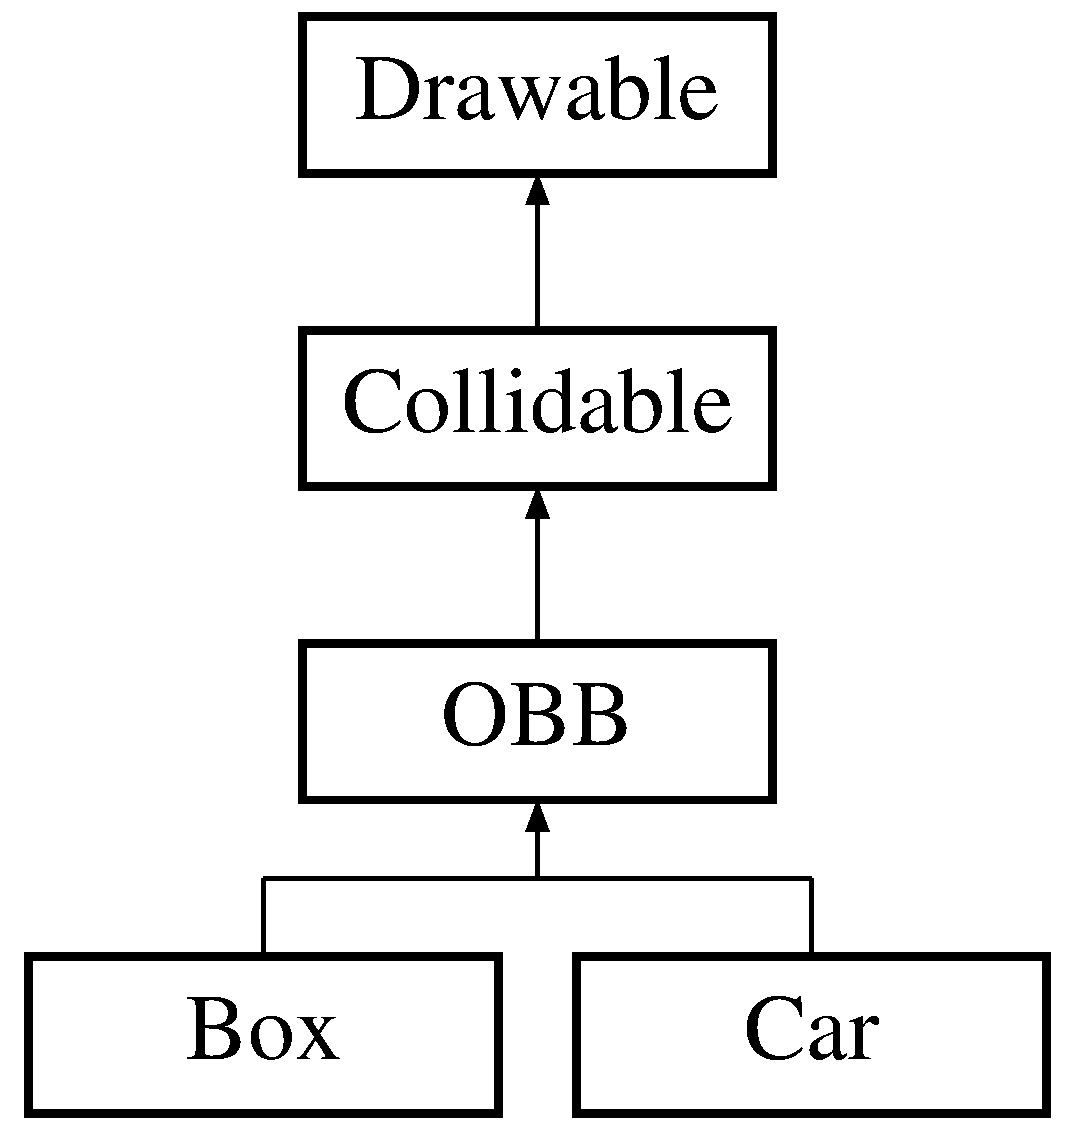
\includegraphics[height=4.000000cm]{class_o_b_b}
\end{center}
\end{figure}
\subsection*{Public Member Functions}
\begin{DoxyCompactItemize}
\item 
\hypertarget{class_o_b_b_a096b260dc12798e724dd9b2f670127f3}{}{\bfseries O\+B\+B} (double f\+Pos\+X, double f\+Pos\+Y, double f\+Half\+Extent\+X, double f\+Half\+Extent\+Y, double f\+Orientation)\label{class_o_b_b_a096b260dc12798e724dd9b2f670127f3}

\item 
\hypertarget{class_o_b_b_a3103d775e6ba4b27a80263ea14826309}{}void {\bfseries update\+Points} ()\label{class_o_b_b_a3103d775e6ba4b27a80263ea14826309}

\item 
\hypertarget{class_o_b_b_acb95cc5ca2f703da43444f6a029d117b}{}\hyperlink{class_vector2_d}{Vector2\+D}$<$ double $>$ {\bfseries get\+Half\+Extents} ()\label{class_o_b_b_acb95cc5ca2f703da43444f6a029d117b}

\item 
\hypertarget{class_o_b_b_a9008e3da97b4e62e47aba521e3a53b61}{}void {\bfseries set\+Half\+Extents} (\hyperlink{class_vector2_d}{Vector2\+D}$<$ double $>$)\label{class_o_b_b_a9008e3da97b4e62e47aba521e3a53b61}

\item 
\hypertarget{class_o_b_b_a2064e40dc401e8c04e3daad5c5aa62d2}{}void \hyperlink{class_o_b_b_a2064e40dc401e8c04e3daad5c5aa62d2}{check\+Collision} (\hyperlink{class_collidable}{Collidable} $\ast$collidable)\label{class_o_b_b_a2064e40dc401e8c04e3daad5c5aa62d2}

\begin{DoxyCompactList}\small\item\em Virtual method to check collision with another \hyperlink{class_collidable}{Collidable} object. \end{DoxyCompactList}\item 
\hypertarget{class_o_b_b_ab55aa6044004c4ea4e5d8310727569c0}{}void \hyperlink{class_o_b_b_ab55aa6044004c4ea4e5d8310727569c0}{check\+Collision} (\hyperlink{class_circle}{Circle} $\ast$circle)\label{class_o_b_b_ab55aa6044004c4ea4e5d8310727569c0}

\begin{DoxyCompactList}\small\item\em Virtual method to check collision with a \hyperlink{class_circle}{Circle} object. \end{DoxyCompactList}\item 
\hypertarget{class_o_b_b_afe394e34d273c0c7b1dfa9a6e28f059f}{}void \hyperlink{class_o_b_b_afe394e34d273c0c7b1dfa9a6e28f059f}{check\+Collision} (\hyperlink{class_o_b_b}{O\+B\+B} $\ast$obb)\label{class_o_b_b_afe394e34d273c0c7b1dfa9a6e28f059f}

\begin{DoxyCompactList}\small\item\em Virtual method to check collision with an \hyperlink{class_o_b_b}{O\+B\+B} object. \end{DoxyCompactList}\item 
\hypertarget{class_o_b_b_a9d0c690a6d3825865b8dd4e023a7cec3}{}void {\bfseries set\+Texture} (sf\+::\+Texture $\ast$texture)\label{class_o_b_b_a9d0c690a6d3825865b8dd4e023a7cec3}

\end{DoxyCompactItemize}
\subsection*{Protected Attributes}
\begin{DoxyCompactItemize}
\item 
\hypertarget{class_o_b_b_a9bb0b948899d85dd6973d7526a574cc2}{}\hyperlink{class_vector2_d}{Vector2\+D}$<$ double $>$ {\bfseries m\+\_\+fv\+Half\+Extents}\label{class_o_b_b_a9bb0b948899d85dd6973d7526a574cc2}

\end{DoxyCompactItemize}
\subsection*{Additional Inherited Members}


The documentation for this class was generated from the following files\+:\begin{DoxyCompactItemize}
\item 
C\+:/\+Users/\+Vitor/\+Documents/\+Visual Studio 2013/\+Projects/\+Course\+Work/coursework/include/\hyperlink{obb_8h}{obb.\+h}\item 
C\+:/\+Users/\+Vitor/\+Documents/\+Visual Studio 2013/\+Projects/\+Course\+Work/coursework/src/\hyperlink{obb_8cpp}{obb.\+cpp}\end{DoxyCompactItemize}

\hypertarget{class_vector2_d}{}\section{Vector2\+D$<$ G $>$ Class Template Reference}
\label{class_vector2_d}\index{Vector2\+D$<$ G $>$@{Vector2\+D$<$ G $>$}}
\subsection*{Public Member Functions}
\begin{DoxyCompactItemize}
\item 
\hypertarget{class_vector2_d_a3bce991141a2cfd9c381651c06d2bee5}{}\hyperlink{class_vector2_d_a3bce991141a2cfd9c381651c06d2bee5}{Vector2\+D} ()\label{class_vector2_d_a3bce991141a2cfd9c381651c06d2bee5}

\begin{DoxyCompactList}\small\item\em Basic constructor that creates an empty vector. \end{DoxyCompactList}\item 
\hypertarget{class_vector2_d_a25ac574bd1a4deb41a9b198afd5f2787}{}\hyperlink{class_vector2_d_a25ac574bd1a4deb41a9b198afd5f2787}{Vector2\+D} (G x, G y)\label{class_vector2_d_a25ac574bd1a4deb41a9b198afd5f2787}

\begin{DoxyCompactList}\small\item\em Constructor that creates and vector with X and Y values. \end{DoxyCompactList}\item 
\hypertarget{class_vector2_d_abbf351182e5d3e725a0b75e82435b846}{}double \hyperlink{class_vector2_d_abbf351182e5d3e725a0b75e82435b846}{dot\+Product} (\hyperlink{class_vector2_d}{Vector2\+D}$<$ G $>$ $\ast$vector2d)\label{class_vector2_d_abbf351182e5d3e725a0b75e82435b846}

\begin{DoxyCompactList}\small\item\em Calculates the dot product of this vector with another one received by reference as a paremeter. \end{DoxyCompactList}\item 
\hypertarget{class_vector2_d_acbe06ed3f1f2360d4826f3914a299aeb}{}\hyperlink{class_vector2_d}{Vector2\+D}$<$ G $>$ {\bfseries subtract} (\hyperlink{class_vector2_d}{Vector2\+D}$<$ G $>$ $\ast$vector2d)\label{class_vector2_d_acbe06ed3f1f2360d4826f3914a299aeb}

\item 
\hypertarget{class_vector2_d_a2c65e6b82fc1879c564850a6f212a588}{}\hyperlink{class_vector2_d}{Vector2\+D}$<$ G $>$ {\bfseries add} (\hyperlink{class_vector2_d}{Vector2\+D}$<$ G $>$ $\ast$vector2d)\label{class_vector2_d_a2c65e6b82fc1879c564850a6f212a588}

\item 
\hypertarget{class_vector2_d_a0dcbc4d12ccef65bf193a52d92fe13b7}{}\hyperlink{class_vector2_d}{Vector2\+D}$<$ G $>$ {\bfseries multiply\+Scalar} (double f\+Scalar)\label{class_vector2_d_a0dcbc4d12ccef65bf193a52d92fe13b7}

\item 
\hypertarget{class_vector2_d_ab87df45d2980f3702f349d2ac7970801}{}\hyperlink{class_vector2_d}{Vector2\+D}$<$ G $>$ {\bfseries divide\+Scalar} (double f\+Scalar)\label{class_vector2_d_ab87df45d2980f3702f349d2ac7970801}

\item 
\hypertarget{class_vector2_d_a1a734dd9f1ca01a88bac3f6bf2be97d0}{}\hyperlink{class_vector2_d}{Vector2\+D}$<$ G $>$ {\bfseries unit\+Vector} ()\label{class_vector2_d_a1a734dd9f1ca01a88bac3f6bf2be97d0}

\item 
\hypertarget{class_vector2_d_af4162d18ba5939bd0175ae01ad6f0221}{}double {\bfseries squared\+Magnitude} ()\label{class_vector2_d_af4162d18ba5939bd0175ae01ad6f0221}

\item 
\hypertarget{class_vector2_d_aab76e76bb642784480bdd231b90b1273}{}double {\bfseries magnitude} ()\label{class_vector2_d_aab76e76bb642784480bdd231b90b1273}

\item 
\hypertarget{class_vector2_d_a85f594928169b9c4bb74cc26ab43d111}{}void {\bfseries rotate} (double f\+Angle)\label{class_vector2_d_a85f594928169b9c4bb74cc26ab43d111}

\item 
\hypertarget{class_vector2_d_a46521876fbb0b52881eba97a074ba59c}{}G {\bfseries get\+X} ()\label{class_vector2_d_a46521876fbb0b52881eba97a074ba59c}

\item 
\hypertarget{class_vector2_d_ac0ecf6cdb4b8106b8c1c2a08efc728df}{}G {\bfseries get\+Y} ()\label{class_vector2_d_ac0ecf6cdb4b8106b8c1c2a08efc728df}

\item 
\hypertarget{class_vector2_d_a6c5526343de1af297d3cc4baca03a9b1}{}void {\bfseries set\+X} (G x)\label{class_vector2_d_a6c5526343de1af297d3cc4baca03a9b1}

\item 
\hypertarget{class_vector2_d_ac7ba076a26efb04c2e590a0cdd3fd20e}{}void {\bfseries set\+Y} (G y)\label{class_vector2_d_ac7ba076a26efb04c2e590a0cdd3fd20e}

\end{DoxyCompactItemize}


The documentation for this class was generated from the following file\+:\begin{DoxyCompactItemize}
\item 
include/\hyperlink{vector2_d_8h}{vector2\+D.\+h}\end{DoxyCompactItemize}

\chapter{File Documentation}
\hypertarget{game_8h}{}\section{C\+:/\+Users/\+Vitor/\+Documents/\+Visual Studio 2013/\+Projects/\+Course\+Work/coursework/include/game.h File Reference}
\label{game_8h}\index{C\+:/\+Users/\+Vitor/\+Documents/\+Visual Studio 2013/\+Projects/\+Course\+Work/coursework/include/game.\+h@{C\+:/\+Users/\+Vitor/\+Documents/\+Visual Studio 2013/\+Projects/\+Course\+Work/coursework/include/game.\+h}}
{\ttfamily \#include \char`\"{}circle.\+h\char`\"{}}\\*
{\ttfamily \#include \char`\"{}collidable.\+h\char`\"{}}\\*
{\ttfamily \#include \char`\"{}collidable\+Factory.\+h\char`\"{}}\\*
{\ttfamily \#include \char`\"{}car.\+h\char`\"{}}\\*
{\ttfamily \#include \char`\"{}tyre.\+h\char`\"{}}\\*
{\ttfamily \#include \char`\"{}vector2\+D.\+h\char`\"{}}\\*
{\ttfamily \#include \char`\"{}rapidxml.\+hpp\char`\"{}}\\*
{\ttfamily \#include \char`\"{}rapidxml\+\_\+iterators.\+hpp\char`\"{}}\\*
{\ttfamily \#include \char`\"{}rapidxml\+\_\+print.\+hpp\char`\"{}}\\*
{\ttfamily \#include \char`\"{}rapidxml\+\_\+utils.\+hpp\char`\"{}}\\*
{\ttfamily \#include $<$array$>$}\\*
{\ttfamily \#include $<$iostream$>$}\\*
{\ttfamily \#include $<$fstream$>$}\\*
{\ttfamily \#include $<$sstream$>$}\\*
{\ttfamily \#include $<$string$>$}\\*
{\ttfamily \#include $<$S\+F\+M\+L/\+Graphics.\+hpp$>$}\\*
\subsection*{Classes}
\begin{DoxyCompactItemize}
\item 
class \hyperlink{class_game}{Game}
\end{DoxyCompactItemize}

\hypertarget{vector2_d_8h}{}\section{include/vector2\+D.h File Reference}
\label{vector2_d_8h}\index{include/vector2\+D.\+h@{include/vector2\+D.\+h}}


Brief explanation.  


\subsection*{Classes}
\begin{DoxyCompactItemize}
\item 
class \hyperlink{class_vector2_d}{Vector2\+D$<$ G $>$}
\end{DoxyCompactItemize}


\subsection{Detailed Description}
Brief explanation. 


\hypertarget{game_8cpp}{}\section{C\+:/\+Users/\+Vitor/\+Documents/\+Visual Studio 2013/\+Projects/\+Course\+Work/coursework/src/game.cpp File Reference}
\label{game_8cpp}\index{C\+:/\+Users/\+Vitor/\+Documents/\+Visual Studio 2013/\+Projects/\+Course\+Work/coursework/src/game.\+cpp@{C\+:/\+Users/\+Vitor/\+Documents/\+Visual Studio 2013/\+Projects/\+Course\+Work/coursework/src/game.\+cpp}}


Implementation of \hyperlink{class_game}{Game} class.  


{\ttfamily \#include \char`\"{}game.\+h\char`\"{}}\\*


\subsection{Detailed Description}
Implementation of \hyperlink{class_game}{Game} class. 


\hypertarget{main_8cpp}{}\section{src/main.cpp File Reference}
\label{main_8cpp}\index{src/main.\+cpp@{src/main.\+cpp}}
{\ttfamily \#include $<$S\+F\+M\+L/\+Graphics.\+hpp$>$}\\*
{\ttfamily \#include \char`\"{}game.\+h\char`\"{}}\\*
{\ttfamily \#include $<$iostream$>$}\\*
{\ttfamily \#include $<$array$>$}\\*
\subsection*{Functions}
\begin{DoxyCompactItemize}
\item 
\hypertarget{main_8cpp_ae66f6b31b5ad750f1fe042a706a4e3d4}{}int {\bfseries main} ()\label{main_8cpp_ae66f6b31b5ad750f1fe042a706a4e3d4}

\end{DoxyCompactItemize}

%--- End generated contents ---

% Index
\backmatter
\newpage
\phantomsection
\clearemptydoublepage
\addcontentsline{toc}{chapter}{Index}
\printindex

\end{document}
